
%proofread!
%issue with spaghetti plot at depth?

\documentclass[jgrga]{agutex}
\usepackage[dvips]{graphicx}
%\usepackage{lineno}
%\linenumbers*[1]

%\noindent $>$latex file \\
%\noindent $>$dvips -P pdf -o file.ps file.dvi \\
%\noindent $>$ps2pdf13 file.ps file.pdf

\authorrunninghead{GUTOWSKI ET AL.}
\titlerunninghead{Radar uncertainty}

\authoraddr{D. Blankenship, Institute for Geophysics, University of Texas at Austin}
\authoraddr{Gail Gutowski, Department of Geosceinces, University of Texas at Austin (gail.gutowski@utexas.edu)}
\authoraddr{Charles S. Jackson, Institute for Geophysics, University of Texas at Austin}
\authoraddr{Duncan Young,  Institute for Geophysics, University of Texas at Austin}


\begin{document}

\title{Uncertainty of ice-penetrating radar and corresponding uncertainty at Byrd Ice Core, Antartica}

\authors{Gail. Gutowski, \altaffilmark{1,2}} Charles S. Jackson, \altaffilmark{2} D. Young, \altaffilmark{2} D. Blankenship, \altaffilmark{2} 

\altaffiltext{1}{Department of Geosciences, University of Texas at Austin, Austin, TX, USA}
\altaffiltext{2}{Institute for Geophysics, University of Texas at Austin, Austin, TX, USA}



\begin{abstract}
Data from radar-sounding surveys of West Antarctica are used to determine the age of observed radar horizons near the Byrd ice core, Antarctica~\citep{gow1968}. We emphasize inclusion of uncertainty in radar- and ice-related sources of uncertainty. The analysis is based on a basic ice-flow model developed by~\citet{schwander2001}. The model assumes no basal melting, zero velocity at the bed, and linear strain rate below 1200 meters depth.

A Bayesian uncertainty analysis is performed to reduce uncertainties and make the best use of the available data. The analysis quantifies observational limitations of the analysis, informing future uncertainty reduction through refinement of observational techniques. A Research Plan outlines a Bayesian approach to develop a new chronology of the Byrd ice core which takes into account theoretical and measurement uncertainties in depth and age of prominent layers observed in the ice column. The method employs Markov Chain Monte Carlo modeling to invert for accumulation and strain as functions of depth. 

ADD: \\
%       where did accum come from?\\
%	comparison to Morley flow?
%	discussion of layers/age deeper in the ice sheet
	add more numbers/tables;\\
	fill out who? references;\\
%	add plenty of references\
%	add bibtex references
%	further description of schwander model?;\\
%	future work
%	discussion of correlation between layers
%	discussion of wa-wa
%	discussion of ECM?
	where did sd's on age come from? -- NOT 3percent!;\\
%	proofread\\
	fix figures \\


\end{abstract}

\begin{article}
\section{Introduction}

The West Antarctic Ice Sheet (WAIS) has become an important focus of glaciological research because it is the last marine ice sheet on Earth. A full 75$\%$ of the ice sheet is based below sea level, leaving the region susceptible to the Marine Ice Sheet Instability Problem \citep{joughin&alley2011}. The problem describes the potential instability of WAIS in the event of grounding line retreat. This process acts as a positive feedback to the system, resulting in accelerated retreat of the grounding line until the ice sheet reaches a steady state position upstream. Marine ice sheet instability could therefore be responsible for a rapid disintegration of up to 75$\%$ of the West Antarctic ice sheet. This scenario would result in a global sea level rise approaching 5m \citep{joughin&alley2011}, threatening tens of millions of individuals worldwide \citep{mcgranahan2007}. It is therefore important to gain a better understanding of ice flow in West Antarctica in order to gauge its susceptibility to catastrophic mass loss in response to climate change.  

Ice-penetrating radar surveys of ice sheets provide a glimpse into the interior of the ice sheet, where other observational methods provide little information. Reflection horizons in the radar reveal the internal isochronous layering of the ice column. Isochronous layers within the ice provide one avenue for developing an understanding of ice dynamics.  Each year, snow accumulates on the surface of the ice sheet. The physical properties of this snow contain information about climatic conditions at the time of deposition. For instance, the oxygen isotope$\delta^{18}O can be used as a proxy for temperature. Over time, the surface layer is covered with the accumulation of subsequent years and becomes buried in the ice column. This process produces isochronous layering within the ice seet which contains information about surface conditions at the time of accumulation of that layer. 
 
For example, the thickness of an isochronous layer which corresponds to the accumulation over the period of deposition of that layer. As the layer is advecting down into the ice sheet, it will thin as a result of gravitational compaction, but it is possible to correct for this effect and so retain some information about accumulation rate. Accumulation rates and patterns of accumulation are related to several climatic factors of interest including air temperature and atmospheric CO$_2$ concentration ~\citep{neftel1988,alley2000}. This makes it possible to recreate ancient climates from long-buried layers of ice. 

These horizons can be tracked over large glaciated regions, in some cases tracing ice flow across hundreds of kilometers, as in the case of West Antarctica ~(\citet[e.g.]{holt2006}). As mentioned earlier, this allows for studies of paleoclimate over large regions of an ice sheet. In East Antarctica, tracking internal layers using ice-penetrating radar presents the opportunity to directly compare ice core analyses between stations located throughout the region. This cross-correlation provides an unprecedented opportunity for constraining the uncertainty of ice core chronologies. 

Some of the latest technology in aerogeophysical surveys of Earth’s major ice sheets includes focused synthetic aperture radar (SAR) techniques. Focused radar products provide an even better picture of glacial isochrones by including additional clutter reduction and preserving echoes from sloped layers. This enhances our ability to detect and track layers, in increasingly more complex englacial environments \citep{peters2006}

It is possible to learn about ice flow from drawdown and deformation observed in the layers. Layer draw down, in which layers move deeper in the glacier (with or without a corresponding change in bed topography) may be indicative of basal melting. In some cases, for example, observations reveal layers disappearing, a sign that ice is (or was) melting. This could correspond to areas of fast-moving ice (past or present) such as an ice stream, or may indicate an area of increased geothermal heating. 

Because internal layering encodes information about accumulation rates and deformation as ice flows, it can be used to develop a picture of ice dynamics. One of the main obstacles in ice sheet modeling is the uncertainty surrounding basal boundary conditions. One way to explore this problem is to use surface observations to invert for basal parameters \citep{thorsteinsson2003}. Dynamical information about the flow of ice within the column, derived from analyses of internal isochrones can further inform these inversion problems to more accurately describe and reduce uncertainties in basal boundary conditions. 


\section{Data}

Radar-echo sounding data was obtained in December 2004 as a part of the Airborne Geophysical Survey of the Amundsen Sea Embayment (AGASEA) project \citep{holt2006}. The radar line passed 870 m from the Byrd ice core site. The plane was travelling at 67 m/s at an elevation of 550 m above the ice. The data includes two-way travel times (the time it takes for a radar pulse to be transmitted, reflect off a layer, and return to the receiver) in microseconds. The data were collected with a 15 MHz bandwidth. We use ten unique layer that were hand picked using GeoFrame because they have some of the strongest reflection amplitudes.

A volcanic chronology was used to quantitatively compare our calculated age-depth relationship to the age of layers in the Byrd ice core \citep{hammer1994}. The chronology was developed using the electrical conductivity method. We used a representative subset of dated volcanic events to cover and age range from 709 BP to more than 18,000 BP. These events correspond to a depth range from 97.8 m to 1890 m below the 1968 surface of the Byrd ice core \citep{gow1968}.

Ice density data as a function of depth were obtained from the original analysis of the ice core \citep{gow1968}. The data were used to account for the varying density of ice in the upper part of the ice sheet. The result was used to apply a firn correction constant to the ice thickness at Byrd ice core. 





\section{Sources of Uncertainty}\label{unc}
There are many sources of uncertainty inherent to the way in which
data is collected, analyzed, and understood. We have included the
following sources of uncertainty.

\subsection{Uncertainty in Radar Two-Way Travel Time (TWTT)}

%As mentioned previously, layers are selected by hand using the program
%GeoFrame. This program allows a user to select strong
%reflectors from a radargram and trace them along a flight
%path. However, there is a fundamental limit to how accurately the
%depth of these layers can be tracked given the resolution of radar
%timing and, in turn, the sampling rate. The sampling rate might be
%anywhere from 5ns to 20ns, so we assume a resolution of 
%10 ns when picking the reflection
%from the surface of the ice sheet and for each internal
%layer. We can then treat the two cases of surface and internal layers
%separately.

%To put this uncertainty into units of depth, we scale the time by
%the velocity of the electromagnetic wave involved. For example, we
%assume the e/m wave travelled to the surface with a velocity of c, the
%speed of light, but then slowed to the velocity of electromagnetic
%radiation in ice, which we assume to be 1.69 x 10$^8$ m/s 
%before reaching the internal layers. This results in a 1$\sigma$ depth
%uncertainty of 0.3 m for the surface and 0.17 m for the internal
%layers. We also consider the fact that the uncertainty picking the
%surface represents a systematic error -- it will be the same for each
%of the internal ice layers. However, the uncertainties of each
%internal layer will not necessarily all be the same, so they should be
%modeled as random within the bounds described above.

%The radar data used for this study was taken using a radar pulse with
%a 15 MHz bandwidth. The limitation of a finite bandwidth means that
%an even an infinitesimally thin layer of ice will appear in the survey
%to have a finite width. To account for this effect, we assume a
%1$\sigma$ depth uncertainty of 5.63 m. This is obtained from considering both
%the bandwidth frequency and the velocity of electromagnetic radiation
%in ice. This uncertainty is applied as a random error for each of our selected
%layers. See Section \ref{method} for additional discussion about how
%all of the sources of uncertainty were included.

There is uncertainty in the picked depth of radar layers.  GeoFrame, seismic interpretation software, allows a user to select strong reflectors from a radargram and trace them along a radar line. However, there is a fundamental limit to how accurate the depth of these layers be given the resolution of the sampling rate of the radar transmitter. This sampling rate reflects the fact that the radar operates by emitting electromagnetic pulses. The receiver then samples the reflections at a given rate. The sampling rate for the data used in this study varies from 5ns to 20ns and so we assume a resolution of 10 ns when picking the reflections from the surface of the ice sheet and from each internal layer. We treat the surface and internal layers separately in this instance. 
	To convert TWTT uncertainty into units of depth, we scale the time by the velocity of electromagnetic wave propagation. For example, we assume the pulse travelled to the surface with velocity, c, the speed of light, but then slowed to the velocity of electromagnetic wave propagation in ice, which we assume to be 1.69 x 108 m/s before reaching the internal layers. The corresponding 1$\sigma$ uncertainty is $\sigma_{surf}$ $\sim$0.3 m for the surface reflector and $\sigma_{lay}~\sim~$0.17 m for the internal layers.  
The uncertainty associated with picking the elevation of the surface is considered a systematic error because the same surface elevation will be used to normalize all of the internal layers. The TWTT uncertainty of each of the internal layers is applied randomly because each of the individual layers need not have the same uncertainty. This is because the reflection from each layer need not have the same phase with respect to the sampling rate. To account for this, we assume the TWTT to be normally distributed and sample randomly from this distribution for each of the internal layers independently.
	The finite bandwidth of the data means that even an infinitesimally thin layer of ice will appear in the survey to have a finite width. Our data used a pulse bandwidth of 15 MHz. This translates to a 1$\sigma$ depth uncertainty of 5.63 m, obtained from considering both the bandwidth frequency and the velocity of electromagnetic radiation in ice. This uncertainty is applied as a random, normally-distributed error in the depth of each of our selected layers. 




\subsection{Uncertainty in determination of age}\label{ageunc}

%Each year fresh snow accumulates on the top of the ice sheet,
%burying the previous season's snowfall. As layers of ice descend into
%the ice sheet, the layers become thinner, as air from the surface is
%squeezed out and gravity compacts the ice. This thinning makes it
%increasingly difficult to distinguish one layer from another at
%depth while in shallow regions, it maybe be possible to simply count
%layers by eye and therefore determine the age of those layers. 

%The uncertainty associated with determining ages for ice layers is a
%function of depth;
%-delta age \\
%-landmarks like 10Be, CH4, F \\
%-ecm method accuracy \\
%-correlation with bc89? \\


	Each year, fresh snow accumulates on top of the ice sheet, burying the previous season’s snowfall. As layers of ice descend into the ice sheet, they become thinner because air is squeezed out and gravity compacts the ice. This thinning makes it increasingly difficult to distinguish one layer from another at depth. In shallow regions, it is possible to count layers by eye to determine the age of near-surface isochrones.\\
	The uncertainty associated with determining ages for ice layers is therefore a function of depth. Several sources are responsible for the increasing uncertainty. There are two methods of dating ice cores: by “ice” age or by “gas” age \citep{bender2006}. This has to do with the fact that ice in the upper part of the glacier still contains atmospheric gases until such a depth as pore closure occurs, squeezing out the air. Because the air is able to penetrate below the surface and into the firn layer, ice at a given depth tends to be older than the air at that depth. This discrepancy leads to an ambiguity in the true age of the ice if atmospheric chemistry is used to determine the age of the ice. Isotopic dating is common among ice core chronologies. Landmark events for concentrations of Beryllium-10, methane, and fluorine (to name a few) are matched to chemical analyses of the ice \citep[e.g.]{schwander2001}. Accepted dates for these events are then mapped onto the ice core. However, there is uncertainty in when these events occurred which needs to be accounted for in the ice core chronology.
	The Electrical Conductivity Method (ECM) is another approach to dating ice. It involves measuring the conductivity of ice at different depths \citep{hammer1994}. This conductivity is associated with the composition of the ice, such as its acidity level. Layers of ash embedded in the ice, for example, will have a distinct conductivity. These ash layers are then attributed to known (or assumed) volcanic events. These events can be related to a volcanic chronology.  However, the volcanic chronology itself has associated uncertainty, which is not well documented. This adds an unknown amount of uncertainty to the ice core chronology.
	Due to the complication of quantifying uncertainty in the Byrd ice core chronology, this analysis assumes an age uncertainty that is 3$\%$ of the documented ice core ages (**NO LONGER DOES***). As age increases deeper in the ice sheet, uncertainty increases accordingly. Follow-up studies will seek to reduce this uncertainty and test for sensitivity of the derived ages to each of the dating methods.





\section{Method}\label{method}
%-firn offset \\
%-depth correction from 1968  \\
%1. determination of depth from radar times \\
%2. use metropolis algorithm to invert for accumlation and ratio of
%surface to basal velocity based on volcanic dating (calculate cost
%based on this) \\
%3. use schwander model to calculate ages (include assumptions)\\


We used an ice model adapted from \citet{schwander2001} to determine the age of internal layers near the Byrd ice core drilling site in Antarctica. We use the model to invert for accumulation and strain rate (assumed constant) as a function of depth.  Input data includes probability distributions of depth for 10 layers near the Byrd ice core site and an age-depth relationship based on volcanic chronology, as discussed previously.
	First, we used a Markov Chain Monte Carlo technique known as the Metropolis algorithm to invert for accumulation and strain rate. The Metropolis algorithm utilizes prior knowledge about hyperparameters (in this case accumulation and strain rate) to step through parameter space. At each step, the algorithm calculates age at every point in the ice column based on the randomly paired hyperparameters.  An associated cost is then calculated  as a measure of the fit of that instance of the model:
\begin{equation}
$$cost = e^\frac{(Age_{model}~ - ~Age_{obs})^2}{(\sigma_{obs})^2}$$
\end{equation}
where $Age_{model}$ is the age distribution of the ten layers calculated by the Schwander model for a given accumulation and strain rate. $Age_{obs}$ and $\sigma_{obs}$ come from the volcanic age-depth function and we allow for the aforementioned uncertainty in $Age_{obs}$ to loosen the constraint on the cost function. At each iteration the algorithm makes a decision about whether or not to accept the combination of hyperparameters based on the cost: if the cost of the nth iteration is less than the cost of the $\textit{(n-1)}$th iteration, the set of parameters is accepted. This means that the nth set of hyperparameters is a better fit to the data (because the cost has decreased). If the cost of the current nth iteration is greater than the cost of the $\textit{(n-1)}$th iteration, the set of parameters is accepted with probability $exp[-\frac{cost_n~-~cost_{n-1}}{2}]$. The algorithm then does a random walk through parameter space, comparing the cost of each step to the step before.
	The Metropolis algorithm uses the principles of Bayesian statistics to generate a large number of distributions that could describe the probability of an outcome. In our case, the outcome is that a radar horizon at a given depth takes on a particular age based on knowledge about ice flow. By generating a large number of sets of parameters (accumulation and strain rate) that define possible ice flow scenarios, it is possible to get a range of ages for each horizon depth. Age uncertainty, in terms of a variance, can be extracted from this distribution of ages.
	With a distribution of ages for every depth in the ice column, we then create depth probability distributions (one for each age distribution we calculated previously) for each of the 10 layers. We assume that all uncertainties can be represented by a gaussian. To find the sampling rate uncertainties, we draw a single value from the probability distribution for the surface reflector, described by $\sigma_{surf}$. We then randomly sample ten values from a probability distribution described by $\sigma_{lay}$, resulting in a radar sampling rate for each of the layers. The bandwidth uncertainty is found in the same fashion as the sampling rate error for the layers, to find a bandwidth depth uncertainty for each of the layers. The bandwidth and latter sampling rate uncertainty vectors are summed.  The sampling rate uncertainty corresponding to the surface is then added to the result. We also add in a correction for firn density and account for additional accumulation between 1968 (when the core was drilled) and 2004 (when the radar line was flown) assuming a constant accumulation rate.
	The result of this process is a single probability distribution for each layer, describing the depth uncertainty for that layer. We then use the forward model of ice flow to find ages (sampled from the previously calculation distribution) that correspond to the range of possible depths of each layer. This gives a range of ages for each layer. The final result is an ensemble of depths and ages for each of the ten prominent radar horizons which take into account uncertainties in both age and depth.






\section{Results}
Figures:
%Histograms of age, depth distributions of piks
%spaghetti plot
%histos of param?
sketch of model in bubbles -- method section
%cost? --don't include
likelihood/model test like morley?

	Our goal is to determine the uncertainty in age and depth of picked radar layers near Byrd Station, West Antarctica through comparison with the Byrd ice core record. Here we show the distribution of age and depth with their modeled uncertainties based on the methods described above. 



Figure~$\ref{depthhist}$ shows the distribution of modeled depths associated with each layer picked from radar observations near Byrd Station, West Antarctica. The spread in the distribution is indicative of limitations in the observation and picking of these layers. Table~$\ref{depths}$ shows the standard deviation of depth for each of the 10 picked layers, assuming the errors to be guassian. See Section~$\ref{ageunc}$ for a full discussion of the sources of uncertainty included in this analysis.




Assuming the resulting age distributions are guassian, the standard deviation of age at each layer is shown in Table $\ref{age}$



Figure~$\ref{spaghetti}$ shows an ensemble of modeled age-depth distributions for the 10 picked radar layers. The distributions are trained on the observed volcanic record at Byrd Station, allowing for uncertainties in both depth and age. Note that both systematic and random sources of uncertainty are included. Crossing lines indicate that random uncertainty plays a significant part in the age-depth distribution of ice layers at Byrd Station. Spread between ensembles that do not cross is representative of systematic uncertainties in the model. 




As described in Section~$\ref{method}$, the model is based on five parameters, layer thickness parameters in four depth regimes and a ratio of surface to bed ice velocity. Figure~$\ref{accum}$ shows the distributions of the layer thickness parameters. We use layer thickness as a proxy for accumulation in the model. As expected due to layer thinning with depth, mean layer thickness decreases with depth. However, our modeled layer thickness overestimates accumulation near Byrd station when compared to the observed ice core record.

For example, surface accumulation near Byrd Station is expected to be about 11 cm/a water-equivalent \citep{who?}; our model estimates a mean **find mean** $\sim$ 0.147 cm/a in the upper part of the ice sheet. ***Insert observed, compare to modeled for rest of regimes **



\section{Discussion and Conclusion}
Uncertainty associated with two-way travel time in airborne ice-penetrating radar surveys of Antarctica is not thoroughly understood. We seek to quantify that uncertainty and its affect on depth and age uncertainties near Byrd Station, West Antarctica. These results will provide an fundamental contribution to the interpretation of ice-penetrating radar observations. Extending the analysis to determine an ensemble of new age-depth distributions near Byrd ice core provides information about dynamic layer deformation in the region. Improved understanding of layer deformation in the Thwaites Glacier catchment (where Byrd Station resides) will contribute to improved ice flow models of the region and a more complete picture of the dynamic history of West Antarctica which will ultimately improve projections of future sea-level rise. 

Our approach employs a simple ice flow model and basic parameter assumptions which we will improve upon in the future. For example, the ice flow model used in this analysis relies heavily on the function of ice accumulation chosen. Here we have chosen to simplify our approach by using layer thickness as a proxy for accumulation. By proposing constant layer thickness in each of four depth regimes, we further approximate accumulation with a discontinuous function. Our depth regimes were selected based on \citet{who?} approximation. While a useful tool, a continuous function of accumulation will be included in the future.

An additional implicit assumption was made about layer independence; each observed ice layer was assumed to have an age and depth independent of the other layers observed in the ice column. In reality, the layers are connected in the system and therefore information learned about on layer may improve our understanding of another neighboring layer. For example, deformation represented by unusual layer thinning in a deep layer will affect the depth of all layers above it. In the future it will be important to explore the influence of such internal ice deformation on our interpretation of the full ice column through correlating the layers. 

One final and fundamental assumption in our analysis is the choice of ice flow model. The model included here was developed for the Dome C region, which generally has slower-moving ice and less accumulation than at Byrd Station \citep{who?}. It will be useful to compare this model to others that are more physically appropriate for Byrd Station and West Antarctica, such as that proposed by \citet{morland}. Assessing the sensitivity of our results on this choice of likelihood will provide an important evaluation of our methods.

%to include:
%layer thickness not as good as accumulation -- overestimating, perhaps problem with %discontinuities
%allow for correlation between layers
%future: include comparison on models (likelihood functions) for comparison





\bibliographystyle{agu}
\bibliography{bib}
\end{article}

%Figures

\begin{figure}
	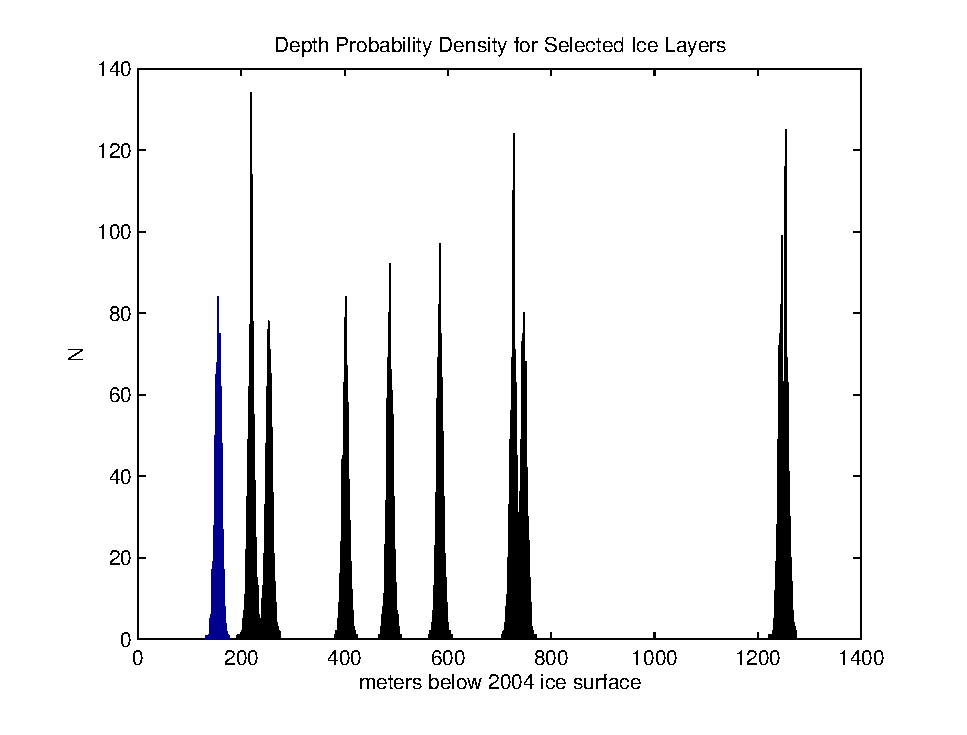
\includegraphics[scale=0.6]{depthhist.eps}
	\label{depthhist}
	\caption{Histogram of modeled water-equivalent ice depth for each of 10 apparently prominent layers observed using airborne radar near Byrd Station, West Antarctica. The width of each distribution is the result of uncertainties arising from the method of radar collection, as discussed in Section~$\ref{method}$.}
\end{figure}

\begin{figure}
	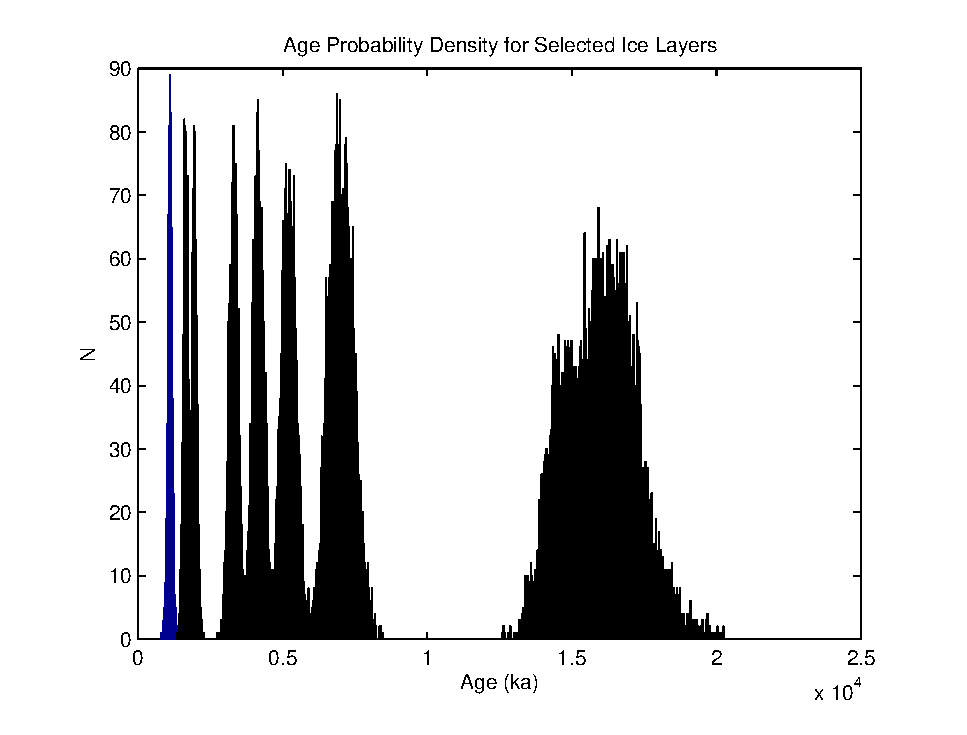
\includegraphics[scale=0.6]{agehist.eps}
	\label{agehist}
	\caption{Histogram of the age distribution for each of 10 prominent layers observed using airborne radar near Byrd Station, West Antarctica. The distribution of ages associated with each layer represents the uncertainty in assigning ages to layers at varying depths. Age uncertainty stems from both radar uncertainty and isotopic ice core dating uncertainties.}
\end{figure}

\begin{figure}
	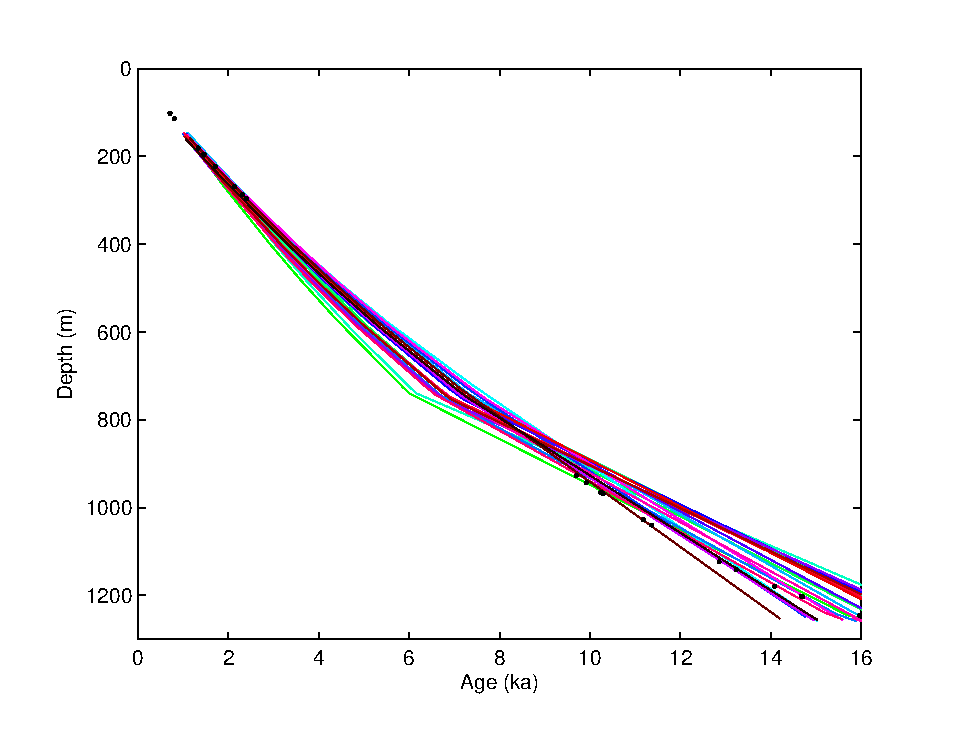
\includegraphics[scale=0.6]{spaghetti_march2012.eps}
	\label{spaghetti}
	\caption{ Modeled age-depth distribution of layers observed using airborne radar near Byrd Station, West Antarctica. Black dots represent isotopically-dated volcanic events from the ice core record at Byrd Station. Each line represents a set of parameters (see Section~$\ref{method}$~that describe the observed data within uncertainty.    }
\end{figure}


\begin{figure}
	\includegraphics{thickgt150.eps}
	\label{accum}
	\caption{Modeled layer thickness in each of four depth regimes near Byrd Station, West Antarctica. **Check what observed is in each of these regimes to compare to mean of distribs** }
\end{figure}
\begin{figure}
	\includegraphics{thickgt1024lt150.eps}
	\label{accum}
	\caption{Modeled layer thickness in each of four depth regimes near Byrd Station, West Antarctica. **Check what observed is in each of these regimes to compare to mean of distribs** }
\end{figure}
\begin{figure}
	\includegraphics{thickgt1294lt150.eps}
	\label{accum}
	\caption{Modeled layer thickness in each of four depth regimes near Byrd Station, West Antarctica. **Check what observed is in each of these regimes to compare to mean of distribs** }
\end{figure}
\begin{figure}
	\includegraphics{thickgt1294.eps}
	\label{accum}
	\caption{Modeled layer thickness in each of four depth regimes near Byrd Station, West Antarctica. **Check what observed is in each of these regimes to compare to mean of distribs** }
\end{figure}

%Tables
%\begin{table}\label{ages}
%\caption{ages}
%\end{table}


%\begin{table*}\label{depths}
%\caption{Time of the Transition Between Phase 1 and Phase 2}%\tablenotemark{a}}
%centering
%\begin{tabular}{l c}
%\hline
% Run  & Time (min)  \\
%\hline
%  $l1$  & 260   \\
%  $l2$  & 300   \\
%  $l3$  & 340   \\
%  $h1$  & 270   \\
%  $h2$  & 250   \\
%  $h3$  & 380   \\
%  $r1$  & 370   \\
%  $r2$  & 390   \\
%\hline
%\end{tabular}
%\tablenotetext{a}{Footnote text here.}
%\end{table*}

\end{document}
